\documentclass{article}

% Language setting
% Replace `english' with e.g. `spanish' to change the document language
\usepackage[english]{babel}

% Set page size and margins
% Replace `letterpaper' with `a4paper' for UK/EU standard size
\usepackage[letterpaper,top=2cm,bottom=2cm,left=3cm,right=3cm,marginparwidth=1.75cm]{geometry}

% Useful packages
\usepackage{amsmath}
\usepackage{graphicx}
\usepackage{mathtools}
\usepackage[colorlinks=true, allcolors=blue]{hyperref}

\title{How to make a good CROT gate}
\author{Tien Nguyen Dinh}

\begin{document}
\maketitle

\begin{abstract}
When we capacitively couple a transmon qubit to a 3D microwave cavity, the cavity inherits a finite nonlinearity from the transmon due to their finite coupling. This nonlinearity is a function of the interrelation among the cavity-transmon detuning $\delta_{ac}$, drive-transmon detuning $\delta_{dc}$, and transmon anharmonicity $\alpha$. Depending on different regimes of parameters, the cavity's nonlinearity varies strongly/weakly. In this work, we look at a system of 5 different modes, namely two bosonic cavities and three transmon qubits. We expect to find a regime in which the self-Kerr $\hat{a}^2, \hat{b}^2$ of the individual cavities is minimized, while the inter-cavity cross-Kerr $\hat{n}_a\hat{n}_b$ is enhanced. The former is important because information stored in a cavity mode with a large self-Kerr tends to be scrambled. The latter is important because it can be leveraged to to make a CROT gate. The said regime is expected to have a as-large-as-possible cross-Kerr profile. That's what makes a good CROT gate.
\end{abstract}

\section{The system Hamiltonian}

Throughout this note, we use the Roman alphabets $a, b$ to denote the cavities, and $c, d, e$ for the transmons. The $c$ letter refers to the middle transmon, coupled to both the cavities (if presented). We \textbf{do} let $\hbar=c=1$. 
We look at a system consisting of three modes first,
\begin{align}
    H &= H_{\text{cav}} + H_{\text{trans}}(t) + H_{\text{int}},\\
    &= \hbar\omega_a a^\dagger a + \underbrace{4E_Cn^2 - E_J\cos\phi -2enV_d\sin(\omega_d t+\theta_d)}_{\text{The transmon + time-dependent drive}} -2enV_a(a+a^\dagger),
\end{align}
where $V_a$ is the strength of the effective voltage fluctuations due to electric field from the cavity mode. We now enter the transmon regime, in which $E_J\gg E_C$. In this regime,
\begin{align}
    H_{\text{trans}} &= 4E_Cn^2 + \frac{1}{2}E_J\phi^2 - E_J(\cos\phi + \frac{1}{2}\phi^2),\\
    &\approx 4E_Cn^2 + \frac{1}{2}E_J\phi^2 - \frac{1}{4!}E_J\phi^4
\end{align}
This truncation is justified because as $E_J/E_C$ increases, the variance of the charge degree of freedom $n$ becomes increasingly large, and simultaneously the variance of the phase degree of freedom $\phi$ becomes increasingly small. In other words, since we work with a very, very specific point of $\phi$ in the transmon regime, only one quartic term $\phi^4$ is enough to approximate the potential at that point. 

Now we introduce the annihilation and creation operators for the transmon, $c$ and $c^\dagger$. They are
\begin{align}
    \phi = (8E_C/E_J)^{1/4}(c+c^\dagger)/\sqrt{2},\\
    n = -i(8E_C/E_J)^{-1/4}(c-c^\dagger)/\sqrt{2}.
\end{align}
It is clear that $[\phi, n]=i$. This makes them look like $[x,p]=i\hbar$. In terms of $c$ and $c^\dagger$, the transmon Hamiltonian reads
\begin{align}
    H_{\text{trans}}(t)/\hbar = \omega_c c^\dagger c - \alpha(c^\dagger+c)^4/12 + (c-c^\dagger)(e^{i\omega_d t}\Omega_d^* - e^{-i\omega_d t}\Omega_d),
\end{align}
where $\hbar\omega_c = \sqrt{8E_CE_J}, \hbar\alpha = E_C, \hbar\Omega_d=eV_de^{-i\theta_d}(8E_C/E_J)^{-1/4}/\sqrt{2}$. We now go into the frame rotate at the drive frequency $\omega_d$ by making a unitary $U=e^{-i(a^\dagger a +c^\dagger c)\omega_d t}$. Using the rotating-wave approximation and the quartic expansion (neglecting terms that do not conserve the excitation number), we arrive at
\begin{align}
    H_{\text{RWA}}/\hbar &= H^{\text{RWA}}_{\text{cav}} + H^{\text{RWA}}_{\text{anc}} + H^{\text{RWA}}_{\text{int}},\\
    &=-\delta_{da}a^\dagger a -\delta_{dc}c^\dagger c - \frac{\alpha}{2}(c^\dagger c+1)c^\dagger c + \Omega_d c^\dagger+\Omega_d^* c+ g_a a c^\dagger + g_a^* a^\dagger c 
\end{align}
In which $\delta_{dx}=\omega_d - \omega_x, x\in\{a, c\}$ and $\hbar g_a=-\sqrt{2}ieV_a(8E_C/E_J)^{-1/4}$.
Now what's the parameter regimes of interest to us? We note that the static part of the system is controlled by two sets of parameters, $r_1=\delta_a/\alpha$ and $r_2 = g_a/\delta_a$. The drive is controlled by $r_3=\delta_d/\alpha$ and $r_4=\Omega_d/\delta_d$. The transmon's anharmonicity $\alpha$ is thus the ultimate parameter that is controlling the Hamiltonian. Lastly, throughout this work, we consider only the regime in which $r_2=g_a/\delta_a$ is much smaller than one. This is the \textit{dispersive regime}. This means $r_2$ is always small. The dispersive regime is desired because it minimizes the hybridization between the cavity modes and the transmon. From a quantum information perspective, the state of the cavity and the linearly coupled transmon is not mixed.

Now, we ask ourselves what are the eigenstates of the $H_{\text{RWA}}$ Hamiltonian. First, in the limit of zero coupling, i.e. $g_a =0$, then the Hamiltonian has only the static part and the driving part. We first make a very very cautious statement: \textit{\textcolor{blue}{The eigenstates of the Hamiltonian $H_{\text{RWA}}$ are product states (verified all traces of $\rho^2$ are unity)}}. In fact, in hindsight this statement is not at all controversal: the drive is purely local, so regardless of the state of the transmon the eigenstates are product states. Ok. Let the product states be $|N_a\rangle\otimes |\psi_m\rangle=|N_a, \psi_m\rangle$ (the cavity's eigenstates are clearly Fock number states). What about $|\psi_m\rangle$? They satisfy the stationary Schrodinger equation,
\begin{align}
    H_{\text{anc}}^{\text{RWA}}|\psi_m\rangle = \epsilon_m|\psi_m\rangle.
\end{align}
Because of the drive, we cannot simply take the eigenstate Fock number $|m\rangle$ of the undriven transmon to be the eigenstates of $H_{\text{anc}}^{\text{RWA}}$. Or can we? Actually, if the drive is turned on slowly enough, then $|m\rangle$ and $|\psi_m\rangle$ are adiabatically connected. Then, we can just label $|N_a, \psi_m\rangle$ as $|n\rangle\otimes |m\rangle$. 

Ok, after labelling $|N_a, \psi_m\rangle$
 as $|n\rangle\otimes |m\rangle$, we try to label the eigenstates of the $H_{\text{RWA}}$ Hamiltonian. We now turn on the coupling $g_a\neq 0$. Then we diagonalize this Hamiltonian,
 \begin{align}\label{eqn:diagHRWA}
     H_{\text{RWA}}=\sum_{m, N_a}\mathcal{E}_m(N_a)|\overline{N_a,\psi_m}\rangle\langle \overline{N_a,\psi_m}|,
 \end{align}
 where $\mathcal{E}_m(N_a)$ are the eigenenergies of the eigenstates $|\overline{N_a,\psi_m}\rangle$ and it can be thought of as an ancilla-state-dependent function of $N_a$. Because of the non-local interaction, the eigenstates of $H_{\text{RWA}}$, whatever they are, are not product states. However, we can play the same card by saying that if the coupling were to be turned on slowly enough, then the state $|\overline{N_a,\psi_m}\rangle$ adiabatically connects to the non-interacting eigenstates $|N_a,\psi_m\rangle$ \textcolor{red}{(Verify this)}. 

To gain further insight into the Hamiltonian in Eqn. (\ref{eqn:diagHRWA}), we introduce operators $A^{(\dagger)} = U_d a^{(\dagger)}U_d^\dagger$. This capital $A^{(\dagger)}$ operator is the unitary transformation of the bare $a^{(\dagger)}$ operator. The unitary $U_d$ is the unitary that diagonalizes the RWA Hamiltonian, i.e. $U_d^\dagger H_{\text{RWA}}U_d$. This is because by construction, we have $|\overline{N_a,\psi_m}\rangle=U_d|N_a,\psi_m\rangle$. And thus
\begin{align}
    H_{\text{RWA}}&=\sum_{m, N_a}\mathcal{E}_m(N_a)U_d|N_a,\psi_m\rangle\langle N_a, \psi_m|U_d^\dagger,\\
    U_d^\dagger H_{\text{RWA}} U_d &= \sum_{m,N_a}\mathcal{E}_m(N_a)|N_a,\psi_m\rangle\langle N_a,\psi_m|.
\end{align}
It should be obvious that $[A, A^\dagger]=1$. The state $|\overline{N_a,\psi_m\rangle}$ is an eigenstate of $A^\dagger A$ with eigenvalue $N_a$. 

\subsubsection{Fitting}

We now perform numerical diagonalization of the full cavity-transmon Hamiltonian to find the strengths of the inherited cavity nonlinearities. We first label the states $|N_a,\psi_m\rangle$. As mentioned, we label them using $|N_a, m\rangle$. After getting $|N_a, m\rangle$ labelled, we next diagonalize the entangled Hamiltonian $(g_a\neq 0)$ again to get the eigenstates $|\overline{N_a,\psi_m}\rangle$. These entangled eigenstates are now labelled using $|N_a,\psi_m\rangle$. Now we go on with the task finding $N_A=A^\dagger A$. In its simplest form, $N_A=U_d a^\dagger U_d^\dagger U_d a U_d^\dagger= U_d a^\dagger a U_d^\dagger$. The problem is that we do not know for sure what is $U_d$. Let's think for a moment, $U_d$ diagonalizes $H_{\text{RWA}}$, meaning that $U_d|N_a,\psi_m\rangle=|\overline{N_a, \psi_m}\rangle$. Then we have
\begin{align}
    U_d &= \sum_{N_a, \psi_m, N_a', \psi'_m} \langle N_a, \psi_m | U_d | N'_a, \psi'_m\rangle|N_a,\psi_m\rangle\langle N'_a, \psi'_m|,\\
    & = \sum_{N_a, \psi_m, N'_a, \psi'_m} \langle N_a, \psi_m | \overline{N'_a, \psi'_m}\rangle |N_a,\psi_m\rangle\langle N'_a, \psi'_m|.
\end{align}
Now that we've obtained $U_d$, we can obtain the ``dressed" creation and annihilation operators readily, $A^{(\dagger)}=U_d(a^{(\dagger)})U_d^\dagger$. The dressed number operator $N_A$ follows immediately. 

Let us now really do the fitting. We approximate the eigenenergies of the Hamiltonian $H_{\text{RWA}}$ as 
\begin{align}\label{eqn:approximatedH}
    \mathcal{E}_m(N_A) = :\delta_{\omega_A, m} N_A+ \frac{K_{A,m}}{2} N_A^2 + \frac{\beta_{A, m}}{3!} N_A^3 + \frac{\sigma_{A,m}}{4!} N_A^4+\dots :
\end{align}
Note that all operators are normal. We are interested only the case $m=0$, i.e. the transmon being in the ground state. 

\subsection{Pseudo-experimental method}

We perform a simulated version of the experiment used to measure Kerr nonlinearities. The experiment goes like this: We first prepare a coherent state $\alpha=1.5$ in the cavity mode and then turn on the off-resonant drive on the transmon. We then let the cavity evolve for some time $\approx 10 \mu$s and measure the cavity Wigner function and then fit this Wigner function to a simulated Wigner function using Lindblad master equation. This allows us to extract the cavity nonlinearities in Eqn. (\ref{eqn:approximatedH}). 

We will modify this protocol a bit. First of all, we will prepare the coherent state using the dressed entangled eigen-basis $\{|\overline{N_a,\psi_m}\rangle\}$. The coherent state is thus 
\begin{align}
    |\beta\rangle = e^{-|\beta|^2/2}\sum_{N_a}\frac{\beta^{N_a}}{\sqrt{N_a !}}|\overline{N_a,\psi_0}\rangle 
\end{align}

\subsubsection{Convergence check}

\begin{figure}
\centering
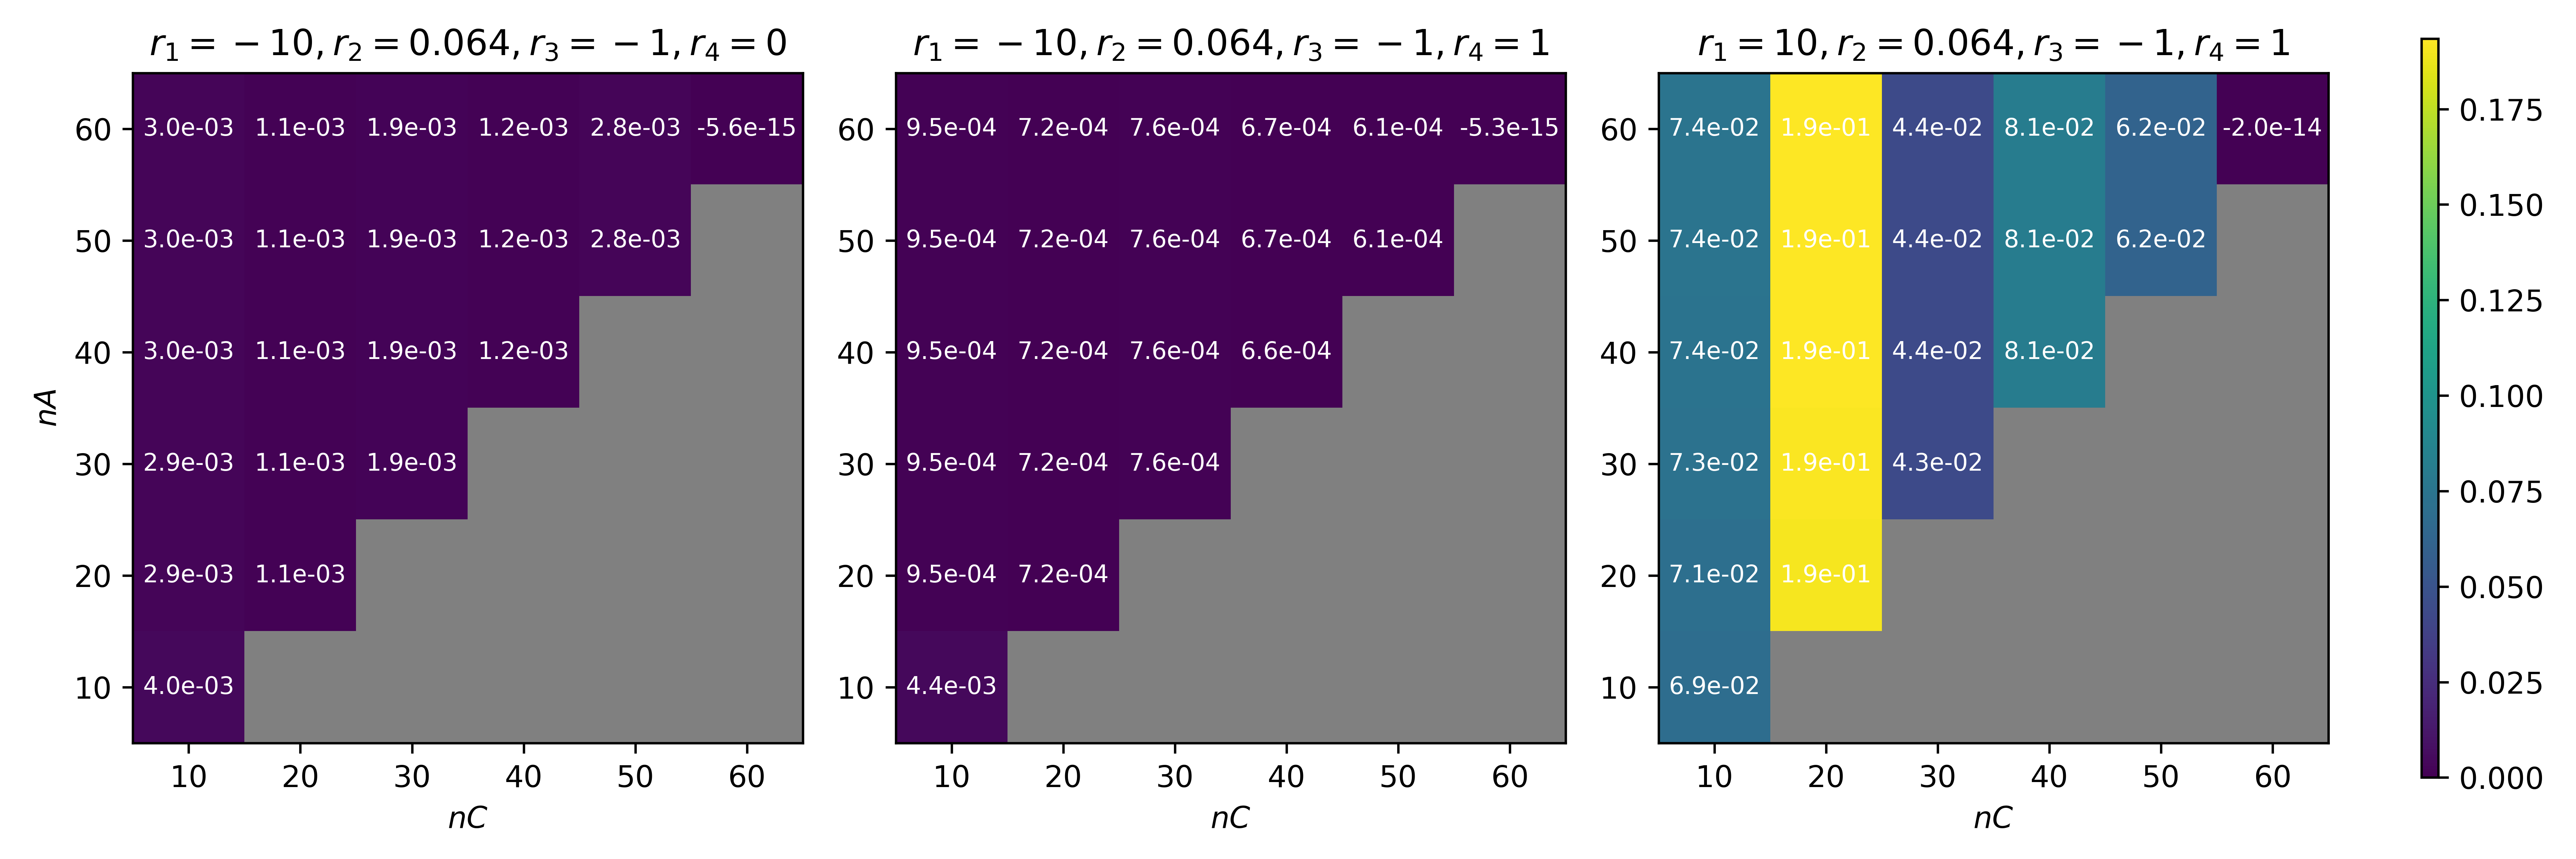
\includegraphics[width=1\linewidth]{truncation_error.png}
\caption{\label{fig:truncation_error}Truncation error for three cases.}
\end{figure}

We need first to check for convergence of our ODE solver \texttt{mesolve}. The system's parameter would be $$\delta_{ac}=10\alpha, 5\alpha, -5\alpha, -10\alpha$$
We keep the absolute difference in the frequency of the cavity and the transmon to be $1$ GHz (thus changing the $\alpha$ value). The drive detuning shall be
$$\delta_{dc}=1\alpha, 0.5\alpha, 0.2\alpha, -0.2\alpha, -0.5\alpha, -1\alpha$$
We pick two special point for the drive amplitude, namely zero drive and unity drive $\Omega_{dc}/\delta_{dc}=0, 1$. The evolution time is taken to be $10\mu$s. First, we create an initial product state $|g, \beta=1.5\rangle$. 

\subsection{A minimal example}

We first look at a minimal example: one cavity mode $a$ coupled to one transmon $c$. We call this the two mode case. The uncoupled Hamiltonian is simply
\begin{align}
    H_0 &= H_{\text{cav}}+H_{\text{anc}},\\
    &=\hbar\omega_a a^\dagger a + 4E_C n^2-E_J\cos\phi,
\end{align}
where $\omega_a$ is the angular frequency of the linear cavity mode; the transmon is completely characterized by the ratio of $E_J/E_C$ and $n$ and $\phi$ are the charge and phase variable as typically referred to in literature \cite{koch07}. We now introduce the drive as a classical field coupled to the charge degree of freedom of the transmon,
\begin{align}
    H_{\text{d}}(t)=-2neV_d\cos(\omega_d t + \theta_d).
\end{align}
The factor $2$ and the minus sign are conventional. $V_d$ is the voltage associated with the classical electric field interacting with the transmon through a dipole-like interaction. Note that $V_d$ has units of voltage $V$, while $e$ has units of Coulomb $C$. The interaction between the two modes is now introduced,
\begin{align}
    H_{\text{int}} &= -2enV_a(a+a^\dagger),\\
    &=\hbar g_a(a+a^\dagger)(c-c^\dagger),
\end{align}
where $V_a$ is the effective voltage fluctuation due to the electric field resides within the cavity and $g$ is the coupling strength between cavity mode and transmon. It is defined to be \begin{align}
    \hbar g_a=-i\sqrt{2}eV_a(8E_C/E_J)^{-1/4}
\end{align}
In other words, the cavity can be thought of as a ``drive" on the transmon qubit.

Now that we have the complete description of the whole system, we would like to see how the system evolve. The description of the whole system is dictated by the Schrodinger equation. Because the Schrodinger equation is a first order linear differential equation, we need one initial condition. Let the condition be $|\psi(t=0)\rangle=\mathcal{N}\left(|\alpha\rangle+|-\alpha\rangle\right)\otimes |0\rangle$. The problem is thus,
\begin{align}
    i\hbar\frac{\text{d}}{\text{d}t}|\psi(t)\rangle = (H_0(t)+H_{\text{int}})|\psi(t)\rangle,\\
    |\psi(t=0)\rangle=\mathcal{N}\left(|\alpha\rangle+|-\alpha\rangle\right)\otimes |0\rangle.
\end{align}
The Schrodinger equation can be solved numerically using \texttt{QuTiP}, either using \texttt{sesolver} or \texttt{mesolver}. Here we omit the influence of decoherence, so \texttt{sesolver} would suffice. We solve the problem for $t$ from $0$ to $60$ $\mu$s. 

\subsubsection{A technical point}

Before we simulate it, we need to find an appropriate representation for the $n$ and $\phi$ operators in the Fock basis. Let us now introduce the corresponding creation and annihilation operators for the transmon, $c^\dagger, c$ such that
\begin{align}
    \phi = (8E_C/E_J)^{1/4}(c+c^\dagger)/\sqrt{2},\\
    n = -i(8E_C/E_J)^{-1/4}(c-c^\dagger)/\sqrt{2}. 
\end{align}
It can be easily seen that $[\phi, n] = i[c, c^\dagger] = i$. For the drive, it is customary to re-write the classical field into its complex representation,
\begin{align}
    E(t) &= V_d\cos(\omega_d t +\theta_d),\\
    &= \frac{V_d}{2}(e^{-i(\omega_d t+\theta_d)}+e^{i(\omega_d t+\theta_d)}),\\
    &=\frac{1}{2}(V_de^{-i\omega_d t}+V_d^*e^{i\omega_d t}),
\end{align}
where $V_d\coloneqq V_de^{-i\theta_d}$. We can also make $V_d$ time-dependent, i.e. pulse shaping, but that's story for another day. The drive Hamiltonian now reads
\begin{align}
    -2neV_d\cos(\omega_d t + \theta_d)&=-2ne\frac{1}{2}(V_de^{-i\omega_d t}+V_d^*e^{i\omega_d t}),\\
    &=-ne(V_de^{-i\omega_d t}+V_d^*e^{i\omega_d t}),\\
    &=-(-i(8E_C/E_J)^{-1/4}(c-c^\dagger)/\sqrt{2})e(V_de^{-i\omega_d t}+V_d^*e^{i\omega_d t}),\\
    &=(\hbar\Omega_de^{-i\omega_d t}-\hbar\Omega_d^*e^{i\omega_d t})(c-c^\dagger),
\end{align}
where $\Omega_d$ is defined as $\hbar\Omega_d\coloneqq ieV_de^{-i\theta_d}(8E_C/E_J)^{-1/4}/\sqrt{2}$ so that $\Omega_d$ has units of (angular) frequency. 

Because we've recast everything into units of frequency, it is natural to also recast $E_J/E_C$-involved terms into units of frequency. From perturbation theory, we have
\begin{align}
    \hbar\omega_c = \sqrt{8E_CE_J},\\
    \hbar\alpha = E_C.
\end{align}
This implies $E_J=\hbar\omega^2_c/8\alpha$. Now we rewrite the whole Hamiltonian in this new formalism
\begin{align}
    H_{\text{tot}}(t)/\hbar = \omega_a a^\dagger a + 4\alpha n^2 - &(\omega_c^2/8\alpha)\cos\phi +(\Omega_de^{-i\omega_d t}-\Omega_d^*e^{i\omega_d t})(c-c^\dagger)\notag\\
    &+g_a(c-c^\dagger)(a+a^\dagger),
\end{align}
where $\omega_a, \omega_c, \alpha, \Omega_d, \omega_d, g$ are all input parameters in units of (angular) frequency. It is desired to take $\alpha$ as the reference value. This, ultimately, makes $E_C$ the reference value. Then the Hamiltonian is controlled by four sets of parameters,
\begin{align}
    r_1 = \frac{\delta_a}{\alpha},\quad r_2 = \frac{\delta_d}{\alpha},\quad r_3 = \frac{\Omega_d}{\delta_d},\quad r_4 = \frac{g_a}{\delta_a}. 
\end{align}

Now it's time to take input parameters. Starting from the baseline, we take $\alpha/2\pi=0.168$ GHz and $\omega_{10}/2\pi=4.936$ GHz for the transmons. Throughout this work, we consider the regime in which $g_a/\delta_a$ is much smaller than one. This is the \textit{dispersive regime}. This means $r_4$ is always small. The dispersive regime is desired because it minimizes the hybridization between the cavity modes and the transmon. From a quantum information perspective, the state of the cavity and the linearly coupled transmon is not mixed. And then we've got $r_1$ and $r_2$. We actually have two distinct regimes here, large and small cavity-transmon detuning $|\delta_a|$. How large and small? We compare it to the transmon's anharmonicity $\alpha$. We first stick to the large regime first, perhaps $r_1=9.64$. Then how about $r_2$ and $r_3$? We'll fix $r_2$ to $0.08$, then we'll do a sweep for $r_3$. 

\subsubsection{Numerical results}

We list here again the input parameters for the Hamiltonian.
\begin{table}[h!]
\centering
\begin{tabular}{|c|c|c|c|c|}
\hline
Case                                                                                                          & $r_1=\delta_a/\alpha$ & $r_2=\delta_d/\alpha$ & $r_3=\Omega_d/\delta_d$ & $r_4=g_a/\delta_a$ \\ \hline
\begin{tabular}[c]{@{}c@{}}Large cavity-transmon detuning,\\ $\omega_{10}=4.936$, $\alpha=0.168$\end{tabular} & 9.64                  & 0.08                  & $r_3$                   & 0.064              \\ \hline
\end{tabular}
\end{table}
To solve the Schrodinger equation, we first diagonalize the uncoupled Hamiltonian $H_0=H_{\text{cav}}+H_{\text{anc}}$. This is essentially because $H_{\text{anc}}$ is not diagonal in the Fock basis. Then we label these eigenstates by comparing the fidelity between them and the basis product state of $|n\rangle\otimes |m\rangle$. Then we turn on the coupling $H_I\neq 0$ and label the coupled states again using the uncoupled states. Using these uncoupled states, we can construct a ``dressed" basis, $|\overline{\psi_{m}, N_a}\rangle$. This dressed basis is used for the construction of the dressed Schrodinger cat state as in Fig. (\ref{fig:wigner1}). The resulting dynamics of the state at three instances $t=0, t=\tau/2, t=\tau$ is plotted in Fig. (\ref{fig:wigner1}). We note that the density matrix is reduced since it is obtained by taking the partial trace of the full density matrix (throwing away the part involving the transmon). This is justified because the transmon is assumed to remain in the ground state $|\psi_0\rangle$ throughout the whole evolution.

\begin{figure}\label{fig:wigner1}
\centering
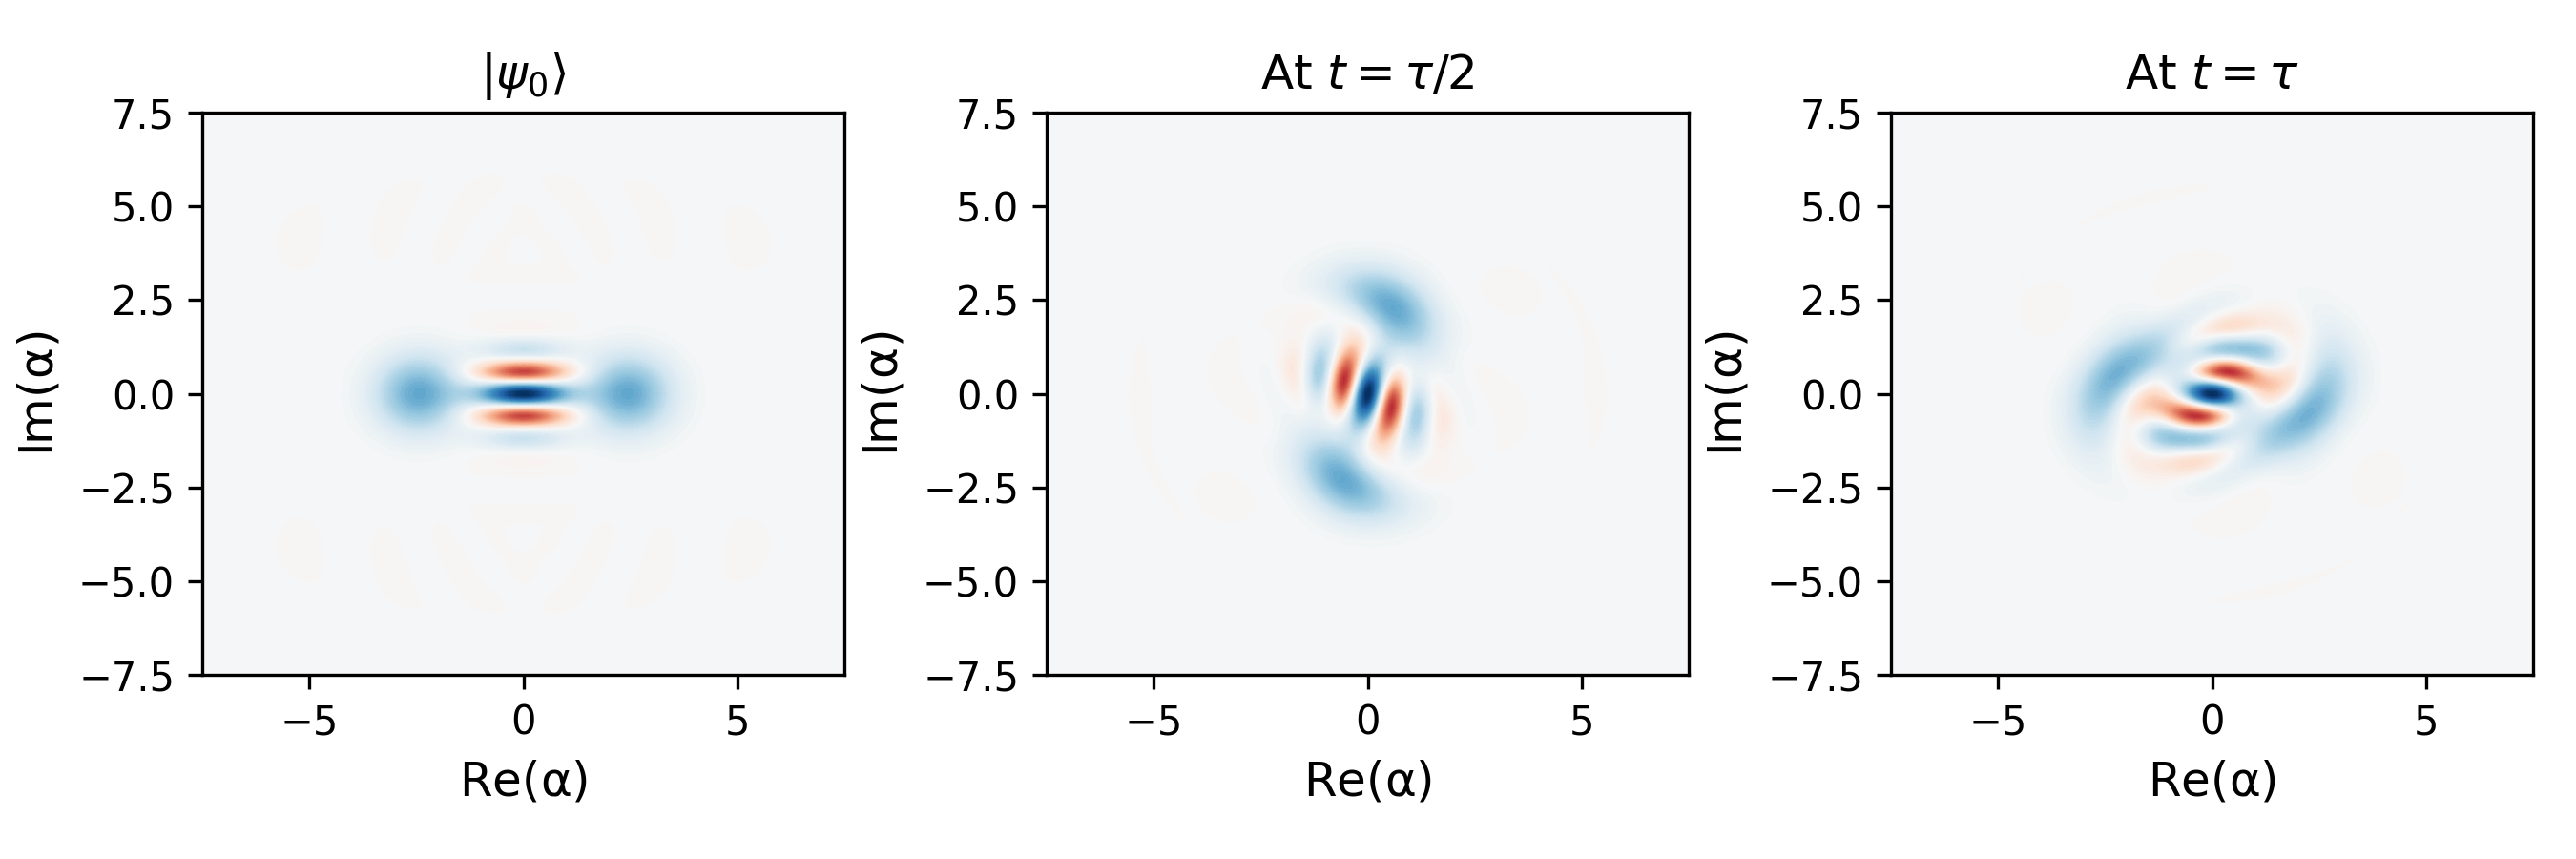
\includegraphics[width=1\linewidth]{wigner1.png}
\caption{\label{fig:frog}This frog was uploaded via the file-tree menu.}
\end{figure}

\subsubsection{Fitted Kerr value}

Based on the resulting dynamics, we can construct a simple Hamiltonian that effectively describing what was going on. The effective Hamiltonian reads
\begin{align}
    H_{\text{eff}} = c_0 + c_1 N_a + c_2 N_a^2 + c_3 N_a^3 + \dots
\end{align}
We stress that this $N_a$ operator is not the usual $a^\dagger a$, but the transformed $U_d (a^\dagger a) U_d^\dagger$ where $U_d$ diagonalizes the full Hamiltonian. We do not in fact have to find $U_d$ because this will be exceedingly hard. Since we have diagonalized the full Hamiltonian and have labelled its eigenstates\footnote{A sanity check would be to see that if $\hat{N}_a|\overline{\psi_0, N_a}\rangle = N_a|\overline{\psi_0, N_a}\rangle$}, the $N_a$ operator is expected to have the form
\begin{align}
    N_a = \sum_{N_a} N_a|\overline{\psi_0, N_a}\rangle\langle\overline{\psi_0, N_a}|.
\end{align}


\section{Some examples to get started}

\subsection{How to create Sections and Subsections}

Simply use the section and subsection commands, as in this example document! With Overleaf, all the formatting and numbering is handled automatically according to the template you've chosen. If you're using the Visual Editor, you can also create new section and subsections via the buttons in the editor toolbar.

\subsection{How to include Figures}

First you have to upload the image file from your computer using the upload link in the file-tree menu. Then use the includegraphics command to include it in your document. Use the figure environment and the caption command to add a number and a caption to your figure. See the code for Figure \ref{fig:frog} in this section for an example.

Note that your figure will automatically be placed in the most appropriate place for it, given the surrounding text and taking into account other figures or tables that may be close by. You can find out more about adding images to your documents in this help article on \href{https://www.overleaf.com/learn/how-to/Including_images_on_Overleaf}{including images on Overleaf}.

\begin{figure}
\centering
\caption{\label{fig:frog}This frog was uploaded via the file-tree menu.}
\end{figure}

\subsection{How to add Tables}

Use the table and tabular environments for basic tables --- see Table~\ref{tab:widgets}, for example. For more information, please see this help article on \href{https://www.overleaf.com/learn/latex/tables}{tables}. 

\begin{table}
\centering
\begin{tabular}{l|r}
Item & Quantity \\\hline
Widgets & 42 \\
Gadgets & 13
\end{tabular}
\caption{\label{tab:widgets}An example table.}
\end{table}

\subsection{How to add Comments and Track Changes}

Comments can be added to your project by highlighting some text and clicking ``Add comment'' in the top right of the editor pane. To view existing comments, click on the Review menu in the toolbar above. To reply to a comment, click on the Reply button in the lower right corner of the comment. You can close the Review pane by clicking its name on the toolbar when you're done reviewing for the time being.

Track changes are available on all our \href{https://www.overleaf.com/user/subscription/plans}{premium plans}, and can be toggled on or off using the option at the top of the Review pane. Track changes allow you to keep track of every change made to the document, along with the person making the change. 

\subsection{How to add Lists}

You can make lists with automatic numbering \dots

\begin{enumerate}
\item Like this,
\item and like this.
\end{enumerate}
\dots or bullet points \dots
\begin{itemize}
\item Like this,
\item and like this.
\end{itemize}

\subsection{How to write Mathematics}

\LaTeX{} is great at typesetting mathematics. Let $X_1, X_2, \ldots, X_n$ be a sequence of independent and identically distributed random variables with $\text{E}[X_i] = \mu$ and $\text{Var}[X_i] = \sigma^2 < \infty$, and let
\[S_n = \frac{X_1 + X_2 + \cdots + X_n}{n}
      = \frac{1}{n}\sum_{i}^{n} X_i\]
denote their mean. Then as $n$ approaches infinity, the random variables $\sqrt{n}(S_n - \mu)$ converge in distribution to a normal $\mathcal{N}(0, \sigma^2)$.


\subsection{How to change the margins and paper size}

Usually the template you're using will have the page margins and paper size set correctly for that use-case. For example, if you're using a journal article template provided by the journal publisher, that template will be formatted according to their requirements. In these cases, it's best not to alter the margins directly.

If however you're using a more general template, such as this one, and would like to alter the margins, a common way to do so is via the geometry package. You can find the geometry package loaded in the preamble at the top of this example file, and if you'd like to learn more about how to adjust the settings, please visit this help article on \href{https://www.overleaf.com/learn/latex/page_size_and_margins}{page size and margins}.

\subsection{How to change the document language and spell check settings}

Overleaf supports many different languages, including multiple different languages within one document. 

To configure the document language, simply edit the option provided to the babel package in the preamble at the top of this example project. To learn more about the different options, please visit this help article on \href{https://www.overleaf.com/learn/latex/International_language_support}{international language support}.

To change the spell check language, simply open the Overleaf menu at the top left of the editor window, scroll down to the spell check setting, and adjust accordingly.

\subsection{How to add Citations and a References List}

You can simply upload a \verb|.bib| file containing your BibTeX entries, created with a tool such as JabRef. You can then cite entries from it, like this: \cite{greenwade93}. Just remember to specify a bibliography style, as well as the filename of the \verb|.bib|. You can find a \href{https://www.overleaf.com/help/97-how-to-include-a-bibliography-using-bibtex}{video tutorial here} to learn more about BibTeX.

If you have an \href{https://www.overleaf.com/user/subscription/plans}{upgraded account}, you can also import your Mendeley or Zotero library directly as a \verb|.bib| file, via the upload menu in the file-tree.

\subsection{Good luck!}

We hope you find Overleaf useful, and do take a look at our \href{https://www.overleaf.com/learn}{help library} for more tutorials and user guides! Please also let us know if you have any feedback using the Contact Us link at the bottom of the Overleaf menu --- or use the contact form at \url{https://www.overleaf.com/contact}.

\section{30 Jul 24: Strategy to implement arbitrary angles}

The CROT gate has to be constructed in a way that it allows arbitrary angle of rotation $\exp(i\varphi\hat{n}_a\otimes\hat{n}_b)$. It's based on the cross-Kerr interaction (cross phase modulation) between the two bosonic modes namely $a$ and $b$,
\begin{align}
    H = -\chi_{ab}\hat{b}^\dagger\hat{a}^\dagger\hat{a}\hat{b}
\end{align}
Now, our scheme seems to imply that $\chi_{ab}$ can be tuned by an off-resonant drive on the transmon mediator. We therefore need to find two working points: on and off.
\bibliographystyle{alpha}
\bibliography{refs}

\end{document}